\documentclass[UTF8]{ctexart}
\usepackage{graphicx}
\usepackage{amsmath}
\usepackage{cite}
\usepackage[a4paper,left=2.5cm,right=2.5cm,top=3cm,bottom=3cm]{geometry}
\title{实验报告}
\author{禤科材 PB20030874 20级14系}
\date{\today}
\bibliographystyle{plain}


\begin{document}
\maketitle
    
    \section{实验目的}
    测量蓖麻油的黏滞系数
    
    \section{实验器材}
    量筒、密度计、温度计、金属球、螺旋测微器、游标卡尺、直尺

    \section{实验原理}

\emph{斯托克斯公式}\cite{jiangyi}

    当半径为 r 的光滑圆球,以速度 V 在均匀的无限宽广的液体中运动时,若速度不大,球也很小,在液
体中不产生涡流的情况下,斯托克斯指出,球在液体中所受到的阻力为
\begin{equation}
    F=6\pi \eta \nu \gamma 
\end{equation}
阻力的大小和物体运动速度成比例,bi
式中F是小球受到的黏滞阻力,
$\eta$为液体的粘度,
$\nu $是小球下落的速度,
$\gamma $是小球的半径。

\emph{雷诺数的修正}\cite{jiangyi}

液体各层间相对运动速度较小时,呈现稳定的运动状态,
如果各层间相对运动较快,就会破坏这种层流,逐渐过渡到湍流,甚至出现漩涡。
故物理学家定义一个无量纲的参数——雷诺数$R_e$来表征液体运动状态的稳定性。
设液体在圆形截面的管中的流速为$\nu$ ,液体的密度为$\rho$ 0,粘度为$\eta$ ,圆管的半径为$r$,则
\begin{equation}
    R_e=\frac{2\nu \rho r}{\eta} 
\end{equation}
于是斯托克斯公式修正如下:
\begin{equation}
    F=6\pi \eta \nu r(1+\frac{3}{16}R_e-\frac{19}{1800}R_e^2...)
\end{equation}

\emph{容器壁的影响}\cite{jiangyi}

在一般情况下,小球仅能在容器半径为$R$、液体高度为$h$的液体内下落,
因此,考虑到容器壁的影响,斯托克斯公式变为:
\begin{equation}
    F=6\pi \eta \nu r(1+2.4\frac{r}{R})(1+3.3\frac{r}{h})(1+\frac{3}{16}R_e-\frac{19}{1800}R_e^2...)
\end{equation}
根据牛顿第一定律,匀速下落的小球受到重力、浮力和黏滞阻力的作用下处于平衡状态,有:



下为不同温度下蓖麻油粘度系数参考表
\begin{figure}[ht]
    \centering 
    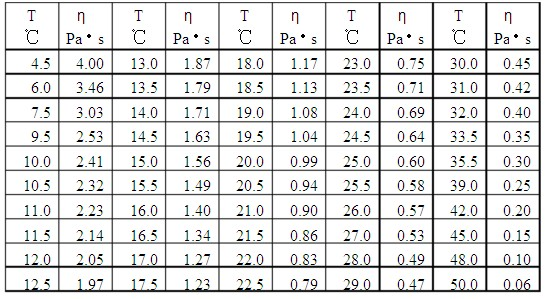
\includegraphics[width=13cm]{standard table.jpeg}
\end{figure}




    \section{测量记录}

    \section{数据处理}

    \section{误差分析}

    \section{提出改进}
    
    \section{思考题}
    2.根据牛顿第二定律,建立微分方程:
    \begin{equation}
        \frac{d^2x}{dt^2}+6\pi\eta r\frac{dx}{dt}=\frac 43 \pi r^3(\rho -\rho _0)g
    \end{equation}

    这是二阶常系数非齐次线性微分方程\cite{shufen}
    
    齐次通解:
    \begin{equation}
        x_1=C_1+C_2e^{-6\pi \eta rt}
    \end{equation}

    非齐次特解:
    \begin{equation}
        x_2=\frac{2r^2(\rho -\rho _0)g}{9\eta}t
    \end{equation}
    
     通解:
    \begin{equation}
        C_1+C_2e^{-6\pi \eta rt}+\frac{2r^2(\rho -\rho _0)g}{9\eta}t 
    \end{equation}

    由方程可见,解由稳态解$\frac{2r^2(\rho -\rho _0)g}{9\eta}t$和衰减解$C_2e^{-6\pi \eta rx}$构成

    由于严格成立的方程(8)并非线性方程,故不失科学性,可设衰减解小于等于给定的小量$\varepsilon $时,可看做匀速运动,故此时$r_1x_1=r_2x_2$。
    舍去衰减解,将路程$s$近似为稳态解$x_2$,作比:
    \begin{equation*}
        \frac{s_1}{s_2}=\frac{r_1}{r_2}
    \end{equation*}

    综上所述,小球半径越大,衰减解衰减越快,但达到稳定速度所需路程越长。所以小球的匀速区间一定是大球的匀速区间,反之则不一定
    
    3.落球法仅对粘度系数较大的透明或半透明液体适用,因为需要能够观察小球的下落的详细情况找出匀速下降区,才能将速度带入公式。如果液体透明度低,应当考虑采用传感器记录小球的下落情况

    4.雷诺数$R_e$是流体力学中表征粘性影响的相似准则数,用以判别粘性流体流动状态的一个无因次数群。雷诺数较小时,粘滞力对流场的影响大于惯性,流场中流速的扰动会因粘滞力而衰减,流体流动稳定,为层流;反之,若雷诺数较大时,惯性对流场的影响大于粘滞力,流体流动较不稳定,流速的微小变化容易发展、增强,形成紊乱、不规则的紊流流场。
    \nocite{daolun}
    \nocite{shiyanjiaocheng}
    \nocite{dawushiyan}
    \bibliography{math}

\end{document}